%!TEX root = ../larxxia.tex

\section{Directly solve linear systems}
\label{sec:dmsls}
\secttoc
\index{linear equation|(}
\index{system|(}

\begin{comment}
\pooliv{p.64--82}  \layiv{\S1.2} \holti{\S1.2}
\end{comment}




The previous \autoref{sec:isle} solved some example systems of linear equations by hand algebraic manipulation.  
We  continue to do so for small systems.  
However, such by-hand solutions are tedious for systems bigger than say four equations in four unknowns.  
For bigger systems with anything from tens to millions of equations---which are typical in applications---we use computers to find solutions because computers are ideal for tedious repetitive calculations.


\subsection{Compute a system's solution}

\begin{quoted}{Gottfried Wilhelm von Leibniz\index{Leibniz, Gottfried}}
It is unworthy of excellent persons to lose hours like slaves in the labour of calculation.
\end{quoted}

Computers primarily deal with numbers, not algebraic equations, so we have to abstract the coefficients of a system into a numerical data structure.
We use matrices and vectors.
\begin{example} 
The first system of \autoref{eg:2eqs2vars:a}
\begin{equation*}
\begin{array}{l} x+y=3\\2x-4y=0 \end{array}
\quad\text{is written}\quad
\underbrace{\begin{bmatrix} 1&1\\2&-4 \end{bmatrix}}_A
\underbrace{\begin{bmatrix} x\\y \end{bmatrix}}_\xv
=\underbrace{\begin{bmatrix} 3\\0 \end{bmatrix}}_\bv .
\end{equation*}
That is, the system \(\begin{cases} x+y=3\\2x-4y=0 \end{cases}\)
is equivalent to \(A\xv=\bv\) for
\begin{itemize}
\item the so-called coefficient matrix \(A=\begin{bmatrix} 1&1\\2&-4 \end{bmatrix}\), 
\item right-hand side vector \(\bv=(3,0)\), and 
\item vector of variables \(\xv=(x,y)\).
\end{itemize}

\end{example}


The beauty of the form \(A\xv=\bv\) is that the numbers involved in the system are abstracted into the matrix~\(A\) and vector~\bv: \script\ handles such numerical matrices and vectors.
\begin{aside}
In this chapter, the two character symbol `\(A\xv\)' is just a shorthand for all the left-hand sides of the linear equations in a system.
\autoref{sec:moaa} then defines a crucial multiplicative meaning to the composite symbol~`\(A\xv\)'. 
\end{aside}%
For some of you, writing a system in this \idx{matrix-vector form} \(A\xv=\bv\) (\autoref{def:matvecsys} below) will appear to be just some mystic rearrangement of symbols---such an interpretation is sufficient for this chapter.
However, those of you who have met matrix multiplication will recognise that \(A\xv=\bv\) is an expression involving natural operations for matrices and vectors: \autoref{sec:moaa} defines and explores such useful operations.

\begin{definition}[matrix-vector form] \label{def:matvecsys}
For every given \idx{system} of \(m\)~\idx{linear equation}s in \(n\)~variables
\begin{eqnarray*}
&&a_{11}x_1+a_{12}x_2+\cdots+a_{1n}x_n=b_1\,,
\\&&a_{21}x_1+a_{22}x_2+\cdots+a_{2n}x_n=b_2\,,
\\&&\quad\vdots
\\&&a_{m1}x_1+a_{m2}x_2+\cdots+a_{mn}x_n=b_m\,,
\end{eqnarray*}
its \bfidx{matrix-vector form} is \(A\xv=\bv\) for the \(m\times n\) \bfidx{matrix} of coefficients
\begin{equation*}
A=\begin{bmatrix} a_{11}&a_{12}&\cdots&a_{1n}
\\a_{21}&a_{22}&\cdots&a_{2n}
\\\vdots&\vdots&\ddots&\vdots
\\a_{m1}&a_{m2}&\cdots&a_{mn} \end{bmatrix},
\end{equation*}
and vectors \(\xv=(\hlist xn)\) and \(\bv=(\hlist bm)\).
If \(m=n\) (the number of equations is the same as the number of variables), then \(A\)~is called a \bfidx{square matrix} (the number of rows is the same as the number of columns).
\end{definition}


\begin{example}[\idx{matrix-vector form}] \label{eg:matvecsys}
Write the following systems in matrix-vector form.
\begin{Parts}
\item \(\begin{array}{l}
x_1+x_2-x_3=-2\,,\\
x_1+3x_2+5x_3=8\,,\\
x_1+2x_2+x_3=1\,.
\end{array}\)

\item \(\begin{array}{l} -2r+3s=6\,,\\s-4t=-\pi\,. \end{array}\)
\end{Parts}
\begin{solution} 
\begin{enumerate}
\item The first system, that of \autoref{eg:3eq3var}, is of three equations in three variables (\(m=n=3\)) and is written in the form \(A\xv=\bv\) as
\begin{equation*}
\underbrace{\begin{bmatrix} 1&1&-1\\ 1&3&5\\1&2&1 \end{bmatrix}}_A
\underbrace{\begin{bmatrix} x_1\\x_2\\x_3 \end{bmatrix}}_\xv
=\underbrace{\begin{bmatrix} -2\\8\\1 \end{bmatrix}}_\bv 
\end{equation*}
for square matrix~\(A\).

\item The second system has three variables called \(r\), \(s\) and~\(t\) and two equations.
Variables `missing' from an equation are represented as zero times that variable, thus the system
\begin{equation*}
\begin{array}{l} -2r+3s+0t=6\,,\\0r+s-4t=-\pi\,, \end{array}
\quad\text{is}\quad
\underbrace{\begin{bmatrix} -2&3&0\\ 0&1&-4 \end{bmatrix}}_A
\underbrace{\begin{bmatrix} r\\s\\t \end{bmatrix}}_\xv
=\underbrace{\begin{bmatrix} 6\\-\pi \end{bmatrix}}_\bv 
\end{equation*}
for \(2\times3\) matrix~\(A\).
\end{enumerate}
\end{solution}
\end{example}



\begin{activity}
Which of the following systems correspond to the matrix-vector equation
\begin{equation*}
\begin{bmatrix} -1&3\\1&2 \end{bmatrix}\begin{bmatrix} u\\w \end{bmatrix}=\begin{bmatrix} 1\\0 \end{bmatrix}?
\end{equation*}
\actposs{\(\begin{matrix} -u+3w=1\\u+2w=0 \end{matrix}\)}
{\(\begin{matrix} -x+3y=1\\x+2y=0 \end{matrix}\)}
{\(\begin{matrix} -u+w=1\\3u+2w=0 \end{matrix}\)}
{\(\begin{matrix} -x+y=1\\3x+2y=0 \end{matrix}\)}
\end{activity}




\begin{procedure}[\bfidx{unique solution}] \label{pro:unisol}
In \script, to solve the matrix-vector system \(A\xv=\bv\) for a \idx{square matrix}~\(A\), use commands listed in \cref{tbl:mtlbpre,tbl:mtlbbasics} to:
\begin{enumerate}
\item form matrix~\(A\) and \idx{column vector}~\(\bv\);
\item check \index{rcond()@\texttt{rcond()}}\verb|rcond(A)| exists and is not too small, \(1\geq\text{good} >10^{-2} >\text{poor} >10^{-4} >\text{bad} >10^{-8} >\text{terrible}\), (\verb|rcond(A)| is always between zero and one inclusive);
\item if \index{rcond()@\texttt{rcond()}}\verb|rcond(A)| both exists and is acceptable, then execute \verb|x=A\b|\index{A\slosh@\texttt{A\slosh}} to compute the solution vector~\(\xv\). 
\end{enumerate}
\end{procedure}

Checking \index{rcond()@\texttt{rcond()}}\verb|rcond(A)| avoids gross mistakes.
% such as  ``Lies My Computer Told Me'' \pooliv{p.83}.
\autoref{sec:svdsgs} discovers what \verb|rcond()| is, and why \verb|rcond()| avoids mistakes.%
\footnote{Interestingly, there are incredibly rare pathological matrices for which even \texttt{rcond()} and~\texttt{A\slosh} do fail us \cite[]{Driscoll07}.  
For example, among \(32\times32\) matrices the probability is about~\(10^{-22}\) of encountering a matrix for which \texttt{rcond()} misleads us by more than a factor of a hundred in using~\texttt{A\slosh}.}
In practice, decisions about acceptability are rarely black and white, and so the qualitative ranges of \verb|rcond()| in \cref{pro:unisol} reflect practical realities.

\begin{quoted}{Jan L.~A. van de Snepscheut\index{van de Snepscheut, Jan L.~A.}}
In theory, there is no difference between theory and practice. 
But, in practice, there is. 
\end{quoted}



\begin{table}
\caption{To realize \autoref{pro:unisol}, and other procedures, we need these basics of \script\ as well as that of \autoref{tbl:mtlbpre}.\index{Matlab@\textsc{Matlab}|textbf}\index{Octave|textbf}} \label{tbl:mtlbbasics}
\hrule
\begin{minipage}{\linewidth}
\begin{itemize}
\item The \idx{floating point} numbers are extended by \index{Inf@\texttt{Inf}|textbf}\verb|Inf|, denoting `\idx{infinity}', and \index{NaN@\texttt{NaN}|textbf}\verb|NaN|, denoting `\idx{not a number}' such as the indeterminate~\(0/0\).
\item \index{[\ldots]@\texttt{[\ldots]}|textbf}\verb|[ ... ; ... ; ... ]| forms both matrices and vectors, or use newlines instead of the semi-colons.
\item \index{rcond()@\texttt{rcond()}|textbf}\verb|rcond(A)|  of a \idx{square matrix}~\(A\) \emph{estimates} the reciprocal of the so-called \idx{condition number} of~\(A\) (defined precisely by \autoref{def:condnum}).
\item \index{A\slosh@\texttt{A\slosh}|textbf}\verb|x=A\b| computes an `answer' to \(A\xv=\bv\)\,---but it may not be a solution unless \verb|rcond(A)| exists and is not small;
\item \index{=@\texttt{=}|textbf}Change one element of an array or vector by assigning a new value with assignments \verb|A(i,j)=...| or \verb|b(i)=...| where \verb|i| and~\verb|j| denote some indices.
\item \index{.^@\texttt{.\^}|textbf}For a vector (or matrix) \verb|t| and an exponent~\verb|p|, the operation \verb|t.^p| computes the \verb|p|th~power of each element in the vector; for example, if \verb|t=[1;2;3;4;5]| then \verb|t.^2| results in \verb|[1;4;9;16;25]|.
\item The function \index{ones()@\texttt{ones()}|textbf}\verb|ones(m,1)| gives a (column) vector of \(m\)~ones, \((1,1,\ldots,1)\).
\item Lastly, always remember that `the answer' by a computer is not necessarily `the solution' of your problem.
\end{itemize}
\end{minipage}
\hrule
\end{table}

\begin{example} \label{eg:3eq3varc}
Use \script\ to solve the system (from \autoref{eg:3eq3var})
\begin{equation*}
\begin{array}{l}
x_1+x_2-x_3=-2\,,\\
x_1+3x_2+5x_3=8\,,\\
x_1+2x_2+x_3=1\,.
\end{array}
\end{equation*}
\begin{solution} 
Begin by writing the system in the abstract matrix-vector form \(A\xv=\bv\) as already done by \autoref{eg:matvecsys}.
%\,: here the system is written
%\begin{equation*}
%\underbrace{\begin{bmatrix} 1&1&-1\\ 1&3&5\\1&2&1 \end{bmatrix}}_A
%\underbrace{\begin{bmatrix} x_1\\x_2\\x_3 \end{bmatrix}}_\xv
%=\underbrace{\begin{bmatrix} -2\\8\\1 \end{bmatrix}}_\bv .
%\end{equation*}
Then the three steps of \autoref{pro:unisol} are the following.
\begin{enumerate}
\item Form matrix~\(A\) and {column vector}~\(\bv\) with the \script\ assignments
\begin{aside}
Beware that the symbol~``\texttt{=}'' in \script\ is a procedural 
assignment of a value---very different in nature to the~``\(=\)'' in 
algebra which denotes \idx{equal}ity.
\end{aside}%
\begin{verbatim}
A=[1 1 -1; 1 3 5; 1 2 1]
b=[-2;8;1]
\end{verbatim}
\autoref{tbl:mtlbbasics} summarizes that in \script: each line is one command; the \verb|=|~symbol assigns the value of the right-hand expression to the variable name of the left-hand side; and the \idx{brackets}~\verb|[ ]| construct both matrices and vectors.
\item Check the value of \verb|rcond(A)|: here it is~\(0.018\) which is in the good range.
\item Since \verb|rcond(A)| is acceptable,  execute \verb|x=A\b| to compute the solution vector~\(\xv=(1,-1,2)\) (and assign it to the variable~\verb|x|, see \autoref{tbl:mtlbbasics}). 
\end{enumerate}
All together that is the four commands
\begin{verbatim}
A=[1 1 -1; 1 3 5; 1 2 1]
b=[-2;8;1]
rcond(A)
x=A\b
\end{verbatim}
\setbox\ajrqrbox\hbox{\qrcode{% solve 3 eqns in 3 vars
A=[1 1 -1; 1 3 5; 1 2 1]
b=[-2;8;1]
rcond(A)
x=A\slosh b
}}%
\marginajrbox%
\ifinQRcodes
Such \idx{qr-code}s in the margin encode these commands for you to possibly scan, copy and paste into \script.
\fi
\end{solution}
\end{example}



\begin{activity}
% for i=1:9999,a=0+round(randn(2)*50); if ismember(abs(det(a)),[1 2 5 10]), break, end, end,  a=a, b=0+round(randn(2,1)*50), x=a\b, a'\b
Use \script\ to solve the system \(7x+8y=42\) and \(32x+38y=57\), to find the answer for \((x,y)\) is
\actposs[4]{\(\begin{bmatrix} 114\\-94.5 \end{bmatrix}\)}
{\(\begin{bmatrix} -94.5\\114 \end{bmatrix}\)}
{\(\begin{bmatrix} 73.5\\342 \end{bmatrix}\)}
{\(\begin{bmatrix} 342\\73.5 \end{bmatrix}\)}
\end{activity}





\begin{example} \label{eg:3eq3vard}
Following the previous \autoref{eg:3eq3varc}, solve each of the two systems:
\begin{Parts}
\item \(\begin{array}{l}
x_1+x_2-x_3=-2\,,\\
x_1+3x_2+5x_3=5\,,\\
x_1-3x_2+x_3=1\,;
\end{array}\)
\item \(\begin{array}{l}
x_1+x_2-x_3=-2\,,\\
x_1+3x_2-2x_3=5\,,\\
x_1-3x_2+x_3=1\,.
\end{array}\)
\end{Parts}

\begin{solution} 
Begin by writing, or at least by imagining, each system in matrix-vector form:
\begin{equation*}
\underbrace{\begin{bmatrix} 1&1&-1\\ 1&3&5\\1&-3&1 \end{bmatrix}}_A
\underbrace{\begin{bmatrix} x_1\\x_2\\x_3 \end{bmatrix}}_\xv
=\underbrace{\begin{bmatrix} -2\\5\\1 \end{bmatrix}}_\bv ;
\quad
\underbrace{\begin{bmatrix} 1&1&-1\\ 1&3&-2\\1&-3&1 \end{bmatrix}}_A
\underbrace{\begin{bmatrix} x_1\\x_2\\x_3 \end{bmatrix}}_\xv
=\underbrace{\begin{bmatrix} -2\\5\\1 \end{bmatrix}}_\bv .
\end{equation*}
As the matrices and vectors are modifications of the previous \autoref{eg:3eq3varc} we reduce typing by modifying the matrix and vector of the previous example (using the ability to change an element in a matrix, see \autoref{tbl:mtlbbasics}).
\begin{enumerate}
\item For the first system execute \verb|A(3,2)=-3| and \verb|b(2)=5|
to see the matrix and vector are now
\begin{verbatim}
A =
     1     1    -1
     1     3     5
     1    -3     1
b =
    -2
     5
     1
\end{verbatim}
Check the value of \verb|rcond(A)|, here \(0.14\) is good.
Then obtain the solution from \verb|x=A\b| with the result
\begin{verbatim}
x =
   -0.6429
   -0.1429
    1.2143
\end{verbatim}
That is, the solution \(\xv=(-0.64,-0.14,1.21)\) to two \idx{decimal places} \twodp.\footnote{The four or five \idx{significant digits} printed by \script\ is effectively exact for most practical purposes.
This book often reports two significant digits as two is enough for most human readable purposes.
When a numerical result is reported to two decimal places, the book indicates this truncation with ``\twodp''.\index{2~d.p.|textbf}}

\item For the second system now execute \verb|A(2,3)=-2| to see the new matrix is the required
\begin{verbatim}
A =
     1     1    -1
     1     3    -2
     1    -3     1
\end{verbatim}
Check: find that \verb|rcond(A)| is zero which is classified as terrible.
Consequently we cannot compute a solution of this second system of linear equations (as in \autoref{fig:3eq3var}(c)).
\end{enumerate}
If we were to try~\verb|x=A\b| in this second system, then \script\ would report\footnote{\autoref{sec:im} introduces that the term \index{singular matrix}`singular' means that the matrix does not have a so-called inverse.  The `working \idx{precision}' is the sixteen \idx{significant digits} mentioned in \autoref{tbl:mtlbpre}.}%
\index{Warning:@\texttt{Warning:}}
\begin{verbatim}
Warning: Matrix is singular to working precision. 
\end{verbatim}
However, we cannot rely on \script\ producing such useful messages: we must use \verb|rcond()| to avoid mistakes.
\end{solution}
\end{example}



\begin{example} \label{eg:5eqns5vars}
Use \script\ to solve the system
\begin{equation*}
\begin{array}{r@{{}={}}r}
x_1-2x_2+3x_3+x_4+2x_5&7\,,\\
-2x_1-6x_2-3x_3-2x_4+2x_5&-1\,,\\
2x_1+3x_2-2x_5&-9\,,\\
-2x_1+x_2&-3\,,\\
-2x_1-2x_2+x_3+x_4-2x_5&5\,.
\end{array}
\end{equation*}

\begin{solution} 
Following \autoref{pro:unisol}, form the corresponding matrix and vector, with appropriate zeros, as
\begin{verbatim}
A=[1  -2   3   1   2
  -2  -6  -3  -2   2
   2   3   0   0  -2
  -2   1   0   0   0
  -2  -2   1   1  -2 ]
b=[7;-1;-9;-3;5]
\end{verbatim}
Check: first find \verb|rcond(A)| is acceptably~\(0.020\), and so then compute the solution via \verb|x=A\b| to find the result
\setbox\ajrqrbox\hbox{\qrcode{% solve 5 eqns in 5 variables
A=[1  -2   3   1   2
  -2  -6  -3  -2   2
   2   3   0   0  -2
  -2   1   0   0   0
  -2  -2   1   1  -2 ]
b=[7;-1;-9;-3;5]
rcond(A)
x=A\slosh b
}}%
\marginajrbox%
\begin{verbatim}
x =
    0.8163
   -1.3673
   -6.7551
   17.1837
    3.2653
\end{verbatim}
that is, the solution \(\xv=(0.82,-1.37,-6.76,17.18,3.27)\) \twodp.
\end{solution}
\end{example}


\begin{example} 
What system of linear equations is represented by the following matrix-vector expression?  and what is the result of using \autoref{pro:unisol} for this system?
\begin{equation*}
\begin{bmatrix} -7&3\\ 7&-5\\1&-2 \end{bmatrix}
\begin{bmatrix} y\\z \end{bmatrix}
=\begin{bmatrix} 3\\-2\\1 \end{bmatrix}.
\end{equation*}

\begin{solution} 
The corresponding system of linear equations is
\begin{equation*}
\begin{array}{l}
-7y+3z=3\,,\\7y-5z=-2\,,\\y-2z=1\,.
\end{array}
\end{equation*}
Invoking \autoref{pro:unisol}:
\begin{enumerate}
\item form matrix~\(A\) and \idx{column vector}~\(\bv\) with
\begin{verbatim}
A=[-7 3; 7 -5; 1 -2]
b=[3;-2;1]
\end{verbatim}
\setbox\ajrqrbox\hbox{\qrcode{% attempt to solve a system
A=[-7 3; 7 -5; 1 -2]
b=[3;-2;1]
rcond(A)
}}%
\marginajrbox%

\item check \verb|rcond(A)|: \script\ gives the message%
\index{square matrix}\index{Error using@\texttt{Error using}}%
\begin{verbatim}
Error using rcond
Input must be a square matrix. 
\end{verbatim}
As \verb|rcond(A)| does not exist, the procedure cannot give a solution.
\end{enumerate}
The reason for the procedure not leading to a solution is that a system of three equations in two variables, as here, generally does not have a solution.
\footnote{If one were to execute \texttt{x=A\slosh b}, then you would find \script\ gives the `answer' \(\xv=(-0.77,-0.73)\) \twodp.
But this answer is not a solution.
Instead this answer has another meaning, often sensibly useful, which is explained by \autoref{sec:asie}.
Using \texttt{rcond()} helps us to avoid confusing such an answer with a solution.}
\end{solution}
\end{example}




\begin{reduce}
\begin{example}[\idx{partial fraction} decomposition] 
Recall that mathematical methods sometimes need to separate a \idx{rational function} into a sum of simpler `partial' fractions.  
For example, for some purposes the fraction \(\frac3{(x-1)(x+2)}\) needs to be written as \(\frac1{x-1}-\frac1{x+2}\)\,.  
Solving linear equations helps: \begin{itemize}
\item here  pose that \(\frac3{(x-1)(x+2)} = \frac A{x-1}+\frac B{x+2}\) for some unknown~\(A\) and~\(B\); 
\item then write the right-hand side over the common denominator,
\begin{eqnarray*}
\frac A{x-1}+\frac B{x+2}
&=&\frac{A(x+2)+B(x-1)}{(x-1)(x+2)}
\\&=&\frac{(A+B)x+(2A-B)}{(x-1)(x+2)}
\end{eqnarray*}
and this equals \(\frac3{(x-1)(x+2)}\) only if both \(A+B=0\) and \(2A-B=3\)\,; 
\item solving these two linear equations gives the required \(A=1\) and \(B=-1\) to determine the decomposition \(\frac3{(x-1)(x+2)}=\frac1{x-1}-\frac1{x+2}\)\,.
\end{itemize}


Now find the \idx{partial fraction} decomposition of \(\frac{-4x^3+8x^2-5x+2}{x^2(x-1)^2}\).
\begin{solution} 
Recalling that repeated factors require extra terms in the decomposition, seek a decomposition of the form
\begin{eqnarray*}&&
\frac A{x^2}+\frac B{x}+ \frac C{(x-1)^2} +\frac D{x-1}
\\&=&\frac{A(x-1)^2+Bx(x-1)^2 +Cx^2+ Dx^2(x-1)} {x^2(x-1)^2}
\\&=&\frac{(B+D)x^3+(A-2B+C-D)x^2+(-2A+B)x+(A)} {x^2(x-1)^2}
\\&=&\frac{-4x^3+8x^2-5x+2}{x^2(x-1)^2}\,.
\end{eqnarray*}
For this last equality to hold for all~\(x\) the coefficients of various powers of~\(x\) must be equal: this leads to the linear equation system
\begin{equation*}
\begin{array}{l}
B+D=-4 \\
A-2B+C-D=8 \\
-2A+B=-5\\
A=2
\end{array}
\iff
\begin{bmatrix} 0&1&0&1
\\1&-2&1&-1
\\-2&1&0&0
\\1&0&0&0 \end{bmatrix}\begin{bmatrix} A\\B\\C\\D \end{bmatrix}
=\begin{bmatrix} -4\\8\\-5\\2 \end{bmatrix}.
\end{equation*}
Either solve by hand or by computer.
\begin{itemize}
\item By hand, the last equation gives \(A=2\) so the third equation then gives \(B=-1\)\,.  
Then the first gives \(D=-3\)\,.  
Lastly, the second then gives \(C=8-2+2(-1)+(-3)=1\)\,.  
That is, the decomposition is
\begin{equation*}
\frac{-4x^3+8x^2-5x+2}{x^2(x-1)^2}
=\frac 2{x^2}-\frac 1{x}+ \frac 1{(x-1)^2} -\frac 3{x-1}
\end{equation*}

\item Using \script, form the matrix and right-hand side with
\begin{verbatim}
a=[0 1 0 1
   1 -2 1 -1
   -2 1 0 0
   1 0 0 0]
b=[-4;8;-5;2]
\end{verbatim}
\setbox\ajrqrbox\hbox{\qrcode{% part frac
a=[0 1 0 1
   1 -2 1 -1
   -2 1 0 0
   1 0 0 0]
b=[-4;8;-5;2]
rcond(a)
ABCD=a\slosh b
}}%
\marginajrbox%
Then solve by checking \verb|rcond(a)|, which at~\(0.04\) is good, and so \verb|ABCD=a\b| finds the answer \((2,-1,1,-3)\).
As before, these coefficients give the decomposition as
\begin{equation*}
\frac{-4x^3+8x^2-5x+2}{x^2(x-1)^2}
=\frac 2{x^2}-\frac 1{x}+ \frac 1{(x-1)^2} -\frac 3{x-1}
\end{equation*}

\end{itemize}
\end{solution}
\end{example}
\end{reduce}





\begin{example}[\texttt{rcond} avoids disaster] \label{eg:infertemp2}
In \autoref{eg:infertemp} an American and a European compared temperatures and using measurements from two days discovered the approximation that the American temperature \(T_A=1.82\,T_E+32.73\) where \(T_E\)~denotes the European temperature.
Continuing the story, three days later they again meet and compare the temperatures they experienced: the American reporting that ``for the last three days it has been \(51^\circ\), \(74^\circ\) and~\(81^\circ\)'', whereas the European reports ``why, I recorded it as \(11^\circ\), \(23^\circ\) and~\(27^\circ\)''.
The marginal figure plots this data with the original two data points, apparently confirming a reasonable linear relationship between the two temperature scales.
\marginpar{%
\begin{tikzpicture}[]
\begin{axis}[footnotesize,width=1.15\marginparwidth
    ,xlabel={European, $T_E$},ylabel={American, $T_A$}
    ,xmin=5,xmax=35,ymin=41,ymax=95]
    \addplot+[only marks] coordinates {
    (26,80) (15,60) (11,51) (23,74) (27,81) };
\end{axis}
\end{tikzpicture}}

Let's fit a polynomial to this temperature data.
\begin{solution}
There are five data points.
Each data point gives us an equation to be satisfied.
This suggests we use linear algebra to determine five coefficients in a formula.
Let's fit the data with the quartic polynomial
\begin{equation}
T_A=c_1+c_2T_E+c_3T_E^2+c_4T_E^3+c_5T_E^4,
\label{eq:infertemp2}
\end{equation}
and use the data to determine the coefficients~\hlist c5\,.
Substituting each of the five pairs of \(T_E\) and~\(T_A\) into this equation gives the five linear equations
\begin{eqnarray*}
60&=&c_1+15c_2+225c_3+3375c_4+50625c_5\,, \\
&\vdots&\\
81&=&c_1+27c_2+729c_3+19683c_4+531441c_5\,.
\end{eqnarray*}
Form these into the matrix-vector equation \(A\cv=\tv_A\) for the unknown coefficients \(\cv=(c_1,c_2,c_3,c_4,c_5)\).
In \script\ the vectors of American temperatures~\(\tv_A\), and the \(5\times5\) matrix~\(A\) are constructed below (recall from \autoref{tbl:mtlbbasics} that \verb|te.^p| computes the \verb|p|th~power of each element in the column vector~\verb|te|).
\setbox\ajrqrbox\hbox{\qrcode{% plot temperatures, and matrix
te=[15;26;11;23;27]
ta=[60;80;51;74;81]
plot(te,ta,'o')
A=[ones(5,1) te te.^2 te.^3 te.^4]
}}%
\marginajrbox%
\begin{verbatim}
te=[15;26;11;23;27]
ta=[60;80;51;74;81]
plot(te,ta,'o')
A=[ones(5,1) te te.^2 te.^3 te.^4]
\end{verbatim}
Then solve for the coefficients using~\verb|c=A\ta| to get
\begin{verbatim}
A =
       1      15     225    3375   50625
       1      26     676   17576  456976
       1      11     121    1331   14641
       1      23     529   12167  279841
       1      27     729   19683  531441
c =
 -163.5469
   46.5194
   -3.6920
    0.1310
   -0.0017
\end{verbatim}
Job done---or is it?
To check, let's plot the predictions of the quartic polynomial~\eqref{eq:infertemp2} with these coefficients.
In \script\ we may plot a graph with the following
\setbox\ajrqrbox\hbox{\qrcode{% plot predicted temperatures
t=linspace(5,35);
plot(t,c(1)+c(2)*t+c(3)*t.^2+c(4)*t.^3+c(5)*t.^4)
ylim([41 95])
}}%
\marginajrbox%
\begin{verbatim}
t=linspace(5,35);
plot(t,c(1)+c(2)*t+c(3)*t.^2+c(4)*t.^3+c(5)*t.^4)
\end{verbatim}
and see a graph like the marginal one.
Disaster: the quartic polynomial relationship is clearly terrible as it is too wavy and nothing like the straight line we know it should be (\(T_A=\frac95T_E+32\)).
\marginpar{%
\begin{tikzpicture}[]
\begin{axis}[footnotesize,width=1.15\marginparwidth
    ,xlabel={European, $T_E$},ylabel={American, $T_A$}
    ,xmin=5,xmax=35,ymin=41,ymax=95]
    \addplot+[only marks] coordinates {
    (26,80) (15,60) (11,51) (23,74) (27,81) };
    \addplot+[domain=5:35,no marks] {
    -163.55+46.519*x-3.6920*x^2+0.13095*x^3-1.6888e-03*x^4
    };
\end{axis}
\end{tikzpicture}
}

The problem is we forgot \verb|rcond|.
In \script\ execute~\verb|rcond(A)| and discover \verb|rcond| is \(3\cdot10^{-9}\).
This value is in the `terrible' range classified by \autoref{pro:unisol}.
Thus the solution of the linear equations must not be used: here the marginal plot indeed shows the solution coefficients are not acceptable.
Always use \verb|rcond| to check for bad systems of linear equations.
\end{solution}
\end{example}

The previous \autoref{eg:infertemp2} also illustrates one of the `rules of thumb' in science and engineering: \emph{for data fitting, avoid using polynomials of degree higher than cubic.}
\footnote{In finance, a `rule of thumb' is to avoid fitting data with anything high-order than straight lines!}


\begin{example}[{Global Positioning System} in space-time] \label{eg:gps3t}
Now recall \autoref{eg:gps2}.
Consider the \gps\ receiver in your smart-phone.
The phone's clock is generally in error; it may only be by a second but the \gps\ needs micro-second \idx{precision}. 
Because of such a timing unknown, five satellites determine our precise position in space \emph{and} time.
% From following code
%[x,y,z]=ndgrid(1:20,1:20,1:20);
%d=sqrt(x.^2+y.^2+z.^2);
%j=find(abs(d-round(d))<1e-9);
%k=find((x(j)<=y(j))&(y(j)<=z(j)));
%j=j(k); length(j)
%k=find(abs(d(j)-20)<=1);k=j(k);
%[x(k) y(k) z(k) d(k)]
% Possible Pythagorean quartets near 20
%    7   14   14   21
%    6   10   15   19
%    8   11   16   21
%    4   13   16   21
%    6    6   17   19
%    1    6   18   19
%    6    9   18   21
%    4    8   19   21
%    4    5   20   21
% Pythagorean quartets making near 6
%j=find(abs(d-6)<0.2);
%k=find((x(j)<=y(j))&(y(j)<=z(j)));
%j=j(k); length(j)
%[x(j) y(j) z(j) d(j)]
%   3   3   4   5.8310
%   2   4   4   6
%   1   3   5   5.9161
%   2   3   5   6.1644
%   1   1   6   6.1644

Suppose at some time (according to our smart-phone) the phone receives from a \gps\ satellite that it is at 3D location \((6,12,23)\)\,Mm (Megametres) and that the signal was sent at a true time~\(0.04\)\,s (seconds) before the phone's time.
But the phone's time is different to the true time by some unknown amount, say~\(t\).
Consequently, the travel time of the signal from the satellite to the phone is actually \(t+0.04\)\,s.
Given the speed of light is \(c=300\)\,Mm/s, this is a distance of \(300(t+0.04)=300t+12\) ---linear in the discrepancy of the phone's clock to the \gps\ clock.
Let \((x,y,z)\) be you and your phone's position in 3D space, then the distance to the satellite is also \(\sqrt{(x-6)^2+(y-12)^2+(z-23)^2}\)\,.
Equating the squares of these two gives one equation
\begin{equation*}
(x-6)^2+(y-12)^2+(z-23)^2=(300t+12)^2.
\end{equation*}
Similarly other satellites give other equations that help determine our position.
But writing ``\(300t\)'' all the time is a bit tedious, so replace it with the new unknown \(w=300t\)\,.

Given your phone also detects that four other satellites broadcast the following position and time information:
\((13,20,12)\) time shift~\(0.04\)\,s before;
\((17,14,10)\) time shift~\(0.033\cdots\)\,s before;
\((8,21,10)\) time shift~\(0.033\cdots\)\,s before; and
\((22,9,8)\) time shift~\(0.04\)\,s before.
Adapting the approach of \autoref{eg:gps2}, use linear algebra to determine your phone's location in space.

\begin{solution} 
Let your unknown position be~\((x,y,z)\) and the unknown time shift to the phone's clock~\(t\) be found from \(w=300t\)\,.
Then the five equations from the five satellites are, respectively,
\begin{eqnarray*}
&&(x-6)^2+(y-12)^2+(z-23)^2=(300t+12)^2=(w+12)^2,
\\&&(x-13)^2+(y-20)^2+(z-12)^2=(300t+12)^2=(w+12)^2,
\\&&(x-17)^2+(y-14)^2+(z-10)^2=(300t+10)^2=(w+10)^2,
\\&&(x-8)^2+(y-21)^2+(z-10)^2=(300t+10)^2=(w+10)^2,
\\&&(x-22)^2+(y-9)^2+(z-8)^2=(300t+12)^2=(w+12)^2.
\end{eqnarray*}
Expand all the squares in these equations:
\begin{eqnarray*}
&&x^2-12x+36+y^2-24y+144+z^2-46z+529\\&&{}=w^2+24w+144\,,
\\&&x^2-26x+169+y^2-40y+400+z^2-24z+144\\&&{}=w^2+24w+144\,,
\\&&x^2-34x+289+y^2-28y+196+z^2-20z+100\\&&{}=w^2+20w+100\,,
\\&&x^2-16x+64+y^2-42y+441+z^2-20z+100\\&&{}=w^2+20w+100\,,
\\&&x^2-44x+484+y^2-18y+81+z^2-16z+64\\&&{}=w^2+24w+144\,.
\end{eqnarray*}
As before, these are a system of \idx{nonlinear equation}s and so outside the remit of the course, but a little algebra brings them within.
Subtract the last equation, say, from each of the first four equations: then \emph{all} of the nonlinear squares of variables cancel leaving a linear system.
Combining the constants on the right-hand side, and moving the \(w\)~terms to the left gives the system of four linear equations
\begin{eqnarray*}
&&32x-6y-30z+0w=-80\,,
\\&&18x-22y-8z+0w=-84\,,
\\&&10x-10y-4z+4w=0\,,
\\&&28x-24y-4z+4w=-20\,.
\end{eqnarray*}
Following \autoref{pro:unisol}, solve this system by forming the corresponding matrix and vector as
\begin{verbatim}
A=[32  -6 -30  0
   18 -22  -8  0
   10 -10  -4  4
   28 -24  -4  4 ]
b=[-80;-84;0;-20]
\end{verbatim}
Check \verb|rcond(A)|: it is acceptably~\(0.023\) so compute the solution via \verb|x=A\b| to find
\setbox\ajrqrbox\hbox{\qrcode{% solve GPS equations
A=[32  -6 -30  0
   18 -22  -8  0
   10 -10  -4  4
   28 -24  -4  4 ]
b=[-80;-84;0;-20]
rcond(A)
x=A\slosh b
}}%
\marginajrbox%
\begin{verbatim}
x =
   2
   4
   4
   9
\end{verbatim}
Hence your phone is at location \((x,y,z)=(2,4,4)\)\,Mm. 
Further, the time discrepancy between your phone and the \gps\ satellites' time is proportional to \(w=9\)\,Mm.
Since \(w=300t\), where \(300\)\,Mm/s is the speed of light, the time discrepancy is \(t=\frac9{300}=0.03\)\,s.
\end{solution}
\end{example}








\subsection{Algebraic manipulation solves systems}
\label{sec:amss}

\begin{quoted}{\cite{Higham1996} [p.195]}
A variant of \textsc{ge} [Gaussian Elimination] was used by the Chinese around the first century \textsc{ad}; the \emph{Jiu Zhang Suanshu} (Nine Chapters of the Mathematical Art) contains a worked example for a system of five equations in five unknowns
\end{quoted}

To solve \idx{linear equation}s with non-square matrices, or with poorly conditioned matrices we need to know many more details about linear algebra.

\Needspace{7\baselineskip}
\begin{aside}
This and the next subsection are not essential, but many further courses currently assume knowledge of the content. 
\cref{thm:fred,thm:feweqns} are convenient to establish in the next subsection, but could alternatively be established using \autoref{pro:gensol}. 
\end{aside}
This subsection systematises the algebraic working of \cref{eg:2eqs2vars,eg:3eq3var}.
The systematic approach empowers by-hand solution of systems of linear equations, together with two general properties on the number of solutions possible.
The algebraic methodology invoked here also reinforces algebraic skills that will help in further courses.

In hand calculations we often want to minimize writing, so the discussion here uses two forms side-by-side for the linear equations: one form with all symbols recorded for best clarity; and beside it, one form where only coefficients are recorded for quickest writing.
Translating from one to the other is crucial even in a computing era as the computer also primarily deals with arrays of numbers, and we must interpret what those arrays of numbers mean in terms of linear equations.

\begin{example} 
Recall the system of linear equations of \autoref{eg:3eq3var}:
\begin{equation*}
\begin{array}{l}
x_1+x_2-x_3=-2\,,\\
x_1+3x_2+5x_3=8\,,\\
x_1+2x_2+x_3=1\,.
\end{array}
\end{equation*}
The first crucial level of abstraction is to write this in the \idx{matrix-vector form}, \autoref{eg:matvecsys},
\begin{equation*}
\underbrace{\begin{bmatrix} 1&1&-1\\ 1&3&5\\1&2&1 \end{bmatrix}}_A
\underbrace{\begin{bmatrix} x_1\\x_2\\x_3 \end{bmatrix}}_\xv
=\underbrace{\begin{bmatrix} -2\\8\\1 \end{bmatrix}}_\bv 
\end{equation*}
A second step of abstraction omits the symbols ``\(\big]\xv=\big[\)''---often we draw a vertical (dotted) line to show where the symbols ``\(\big]\xv=\big[\)'' were, but this line is not essential and the theoretical statements ignore such a drawn line.
Here this second step of abstraction represents this linear system by the so-called \idx{augmented matrix}
\begin{equation*}
\begin{bmatrix} 1&1&-1\V -2\\ 1&3&5\V 8\\1&2&1\V 1 \end{bmatrix}
\end{equation*}
\end{example}


\begin{definition} \label{def:augmat}
The \bfidx{augmented matrix} of the \idx{system} of \idx{linear equation}s \(A\xv=\bv\) is the matrix \(\begin{bmatrix} A\V \bv \end{bmatrix}\).
\end{definition}

\begin{example} 
Write down augmented matrices for the two following systems:
\begin{Parts}
\item \(\begin{array}{l} -2r+3s=6\,,\\s-4t=-\pi\,, \end{array}\)
\item \(\begin{array}{l}
-7y+3z=3\,,\\7y-5z=-2\,,\\y-2z=1\,.
\end{array}\)
\end{Parts}
\begin{solution} 
\begin{eqnarray*}
\begin{cases} -2r+3s=6\\s-4t=-\pi \end{cases}
&\iff&%\leftrightarrow&
\begin{bmatrix} -2&3&0\V6\\ 0&1&-4\V-\pi \end{bmatrix}
\\
\begin{cases}
-7y+3z=3\\7y-5z=-2\\y-2z=1
\end{cases}
&\iff&%\leftrightarrow&
\begin{bmatrix} -7&3\V3\\ 7&-5\V-2\\1&-2\V1 \end{bmatrix}
\end{eqnarray*} 
An \idx{augmented matrix} is not unique: it depends upon the order of the equations, and also upon the order you choose for the variables in~\xv.  
The first example implicitly chose \(\xv=(r,s,t)\); if instead we choose to order the variables as \(\xv=(s,t,r)\), then  
\begin{equation*}
\begin{cases} 3s-2r=6\\s-4t=-\pi \end{cases}
\iff%\leftrightarrow
\begin{bmatrix} 3&0&-2\V6\\ 1&-4&0\V-\pi \end{bmatrix}
\end{equation*} 
Such variations to the augmented matrix are valid, but you must remember your corresponding chosen order of the variables.
\end{solution}
\end{example}


\begin{activity}
Which of the following \emph{cannot} be an \idx{augmented matrix} for the system \(p+4q=3\) and \(-p+2q=-2\)\,?
\actposs{\(\begin{bmatrix} 2&-1\V3\\4&1\V-2 \end{bmatrix}\)}
{\(\begin{bmatrix} 1&4\V3\\-1&2\V-2 \end{bmatrix}\)}
{\(\begin{bmatrix} -1&2\V-2\\1&4\V3 \end{bmatrix}\)}
{\(\begin{bmatrix} 4&1\V3\\2&-1\V-2 \end{bmatrix}\)}
\end{activity}





Recall that \cref{eg:2eqs2vars,eg:3eq3var} manipulate the linear equations to deduce solution(s) to systems of linear equations.
The following theorem validates such manipulations in general, and gives the basic operations a collective name. 


\begin{theorem} \label{thm:erowop} 
The following \bfidx{elementary row operation}s can be performed on either a \idx{system} of \idx{linear equation}s or on its corresponding \idx{augmented matrix} without changing the solutions:
\begin{enumerate}
\item \index{interchanging two rows}interchange two equations\slash rows; or
\item multiply an equation\slash row by a nonzero constant; or
\item add a multiple of an equation\slash row to another.
\end{enumerate}
\end{theorem}

\begin{comment}
Interestingly, some other texts omit a proof that row operations preserve the solution(s).  Poole comments on reversibility.  Larson comments that row operations produce `equivalent' systems, but does not prove.  Beezer proves it.
\end{comment}

\begin{proof} 
We just address the system of equations form as the augmented matrix form is equivalent but more abstract.
\begin{enumerate}
\item Swapping the order of two equations does not change the system of equations, the set of relations between the variables, so does not change the solution.
\item Let vector~\xv\ satisfy \(\lincomb axn=b\)\,.
Then \(\lincomb{ca}xn=c(\lincomb axn)=cb\) and so~\xv\ satisfies \(c\)~times the equation.
When the constant~\(c\) is nonzero, the above can be reversed through dividing by~\(c\).
Hence multiplying an equation by a nonzero constant~\(c\) does not change the possible solutions.
\item 
Let vector~\xv\ satisfy both \(\lincomb axn=b\) and \(\lincomb{a'}xn=b'\).
Then
\begin{eqnarray*}
&&(a'_1+ca_1)x_1+(a'_2+ca_2)x_2+\cdots+(a'_n+ca_n)x_n
\\&=&a'_1x_1+ca_1x_1+a'_2x_2+ca_2x_2+\cdots+a'_nx_n+ca_nx_n
\\&=&\lincomb{a'}xn +c(\lincomb{a}xn)
\\&=&b'+cb\,.
\end{eqnarray*}
That is, \xv~also satisfies the equation formed by adding \(c\)~times the first to the second.
Conversely, every vector~\xv\ that satisfies both \(\lincomb axn=b\) and \((a'_1+ca_1)x_1+(a'_2+ca_2)x_2+\cdots+(a'_n+ca_n)x_n=b'+cb\), by adding \((-c)\)~times the first to the second as above, also satisfies \(\lincomb{a'}xn=b'\).
Hence adding a multiple of an equation to another does not change the possible solutions.
\end{enumerate}
\end{proof}



\begin{example} \label{eg:erowops}
Use \idx{elementary row operation}s to find the only solution of the following system of linear equations:
\begin{equation*}
\begin{array}{l}
x+2y+z=1\,,\\ 2x-3y=2\,,\\ -3y-z=2\,.
\end{array}
\end{equation*}
Confirm with \script.
\begin{solution} 
In order to know what the row operations should find, let's first solve the system with \script\ via \autoref{pro:unisol}. 
In matrix-vector form the system is
\begin{equation*}
\begin{bmatrix} 1&2&1\\2&-3&0\\0&-3&-1 \end{bmatrix}
\begin{bmatrix} x\\y\\z \end{bmatrix}
=\begin{bmatrix} 1\\2\\2 \end{bmatrix};
\end{equation*}
hence in \script\ execute
\begin{verbatim}
A=[1 2 1;2 -3 0;0 -3 -1]
b=[1;2;2]
rcond(A)
x=A\b
\end{verbatim}
\setbox\ajrqrbox\hbox{\qrcode{% solve 3 eqns in 3 variables
A=[1 2 1;2 -3 0;0 -3 -1]
b=[1;2;2]
rcond(A)
x=A\slosh b
}}%
\marginajrbox%
\verb|rcond(A)| is just good,~\(0.0104\), so the computed answer \(\xv=(x,y,z)=(7,4,-14)\) is the solution.

Second, use elementary row operations.
Let's write the working in both full symbolic equations and in augmented matrix form in order to see the correspondence between the two---you would not have to do both, either one would suffice.
\begin{eqnarray*}
\begin{cases}
x+2y+z=1\\ 2x-3y+0z=2\\ 0x-3y-z=2
\end{cases}
&\iff&%\leftrightarrow&
\begin{bmatrix} 1&2&1\V1\\2&-3&0\V2\\0&-3&-1\V2 \end{bmatrix}
\\[0ex plus 1ex]
\parbox{0.5\linewidth}{Add \((-2)\) times the first equation\slash row to the second.}
\\[0ex plus 1ex]
\begin{cases}
x+2y+z=1\\ 0x-7y-2z=0\\ 0x-3y-z=2
\end{cases}
&\iff&%\leftrightarrow&
\begin{bmatrix} 1&2&1\V1\\0&-7&-2\V0\\0&-3&-1\V2 \end{bmatrix}
\\[0ex plus 1ex]
\parbox{0.5\linewidth}{This makes the first column have a leading one (\autoref{def:rref}).  Start on the second column by dividing the second equation\slash row by~\((-7)\).}
\\[0ex plus 1ex]
\begin{cases}
x+2y+z=1\\ 0x+y+\frac27z=0\\ 0x-3y-z=2
\end{cases}
&\iff&%\leftrightarrow&
\begin{bmatrix} 1&2&1\V1\\0&1&\frac27\V0\\0&-3&-1\V2 \end{bmatrix}
\\[0ex plus 1ex]
\parbox{0.5\linewidth}{Now subtract twice the second equation\slash row from the first, and add three times the second to the third.}
\\[0ex plus 1ex]
\begin{cases}
x+0y+\frac37z=1\\ 0x+y+\frac27z=0\\ 0x+0y-\frac17z=2
\end{cases}
&\iff&%\leftrightarrow&
\begin{bmatrix} 1&0&\frac37\V1\\0&1&\frac27\V0\\0&0&-\frac17\V2 \end{bmatrix}
\\[0ex plus 1ex]
\parbox{0.5\linewidth}{This makes the second column have the second leading one (\autoref{def:rref}).  
Start on the third column by multiplying the third equation\slash row by~\((-7)\).}
\\[0ex plus 1ex]
\begin{cases}
x+0y+\frac37z=1\\ 0x+y+\frac27z=0\\ 0x+0y+z=-14
\end{cases}
&\iff&%\leftrightarrow&
\begin{bmatrix} 1&0&\frac37\V1\\0&1&\frac27\V0\\0&0&1\V-14 \end{bmatrix}
\\[0ex plus 1ex]
\parbox{0.5\linewidth}{Now subtract \(3/7\)~of the third equation\slash row from the first, and \(2/7\) from the second.}
\\[0ex plus 1ex]
\begin{cases}
x+0y+0z=7\\ 0x+y+0z=4\\ 0x+0y+z=-14
\end{cases}
&\iff&%\leftrightarrow&
\begin{bmatrix} 1&0&0\V7\\0&1&0\V4\\0&0&1\V-14 \end{bmatrix}
\end{eqnarray*}
This completes the transformation of the equations\slash augmented matrix into a so-called \idx{reduced row echelon form} (\autoref{def:rref}).
From this form we read off the solution:  the system of equation on the left directly gives \(x=7\)\,, \(y=4\) and \(z=-14\)\,, that is, the solution vector \(\xv=(x,y,z)=(7,4,-14)\) (as computed by \script);
the transformed augmented matrix on the right tells us exactly the same thing because (\autoref{def:augmat}) it means the same as the matrix-vector 
\begin{equation*}
\begin{bmatrix} 1&0&0\\0&1&0\\0&0&1 \end{bmatrix}
\begin{bmatrix} x\\y\\z \end{bmatrix}
=\begin{bmatrix} 7\\4\\-14 \end{bmatrix},
\end{equation*}
which is the same as the system on the above-left and tells us the solution \(\xv=(x,y,z)=(7,4,-14)\).
\end{solution}
\end{example}





\begin{definition} \label{def:rref} 
 A system of \idx{linear equation}s or \index{augmented matrix}(augmented) matrix is in \bfidx{reduced row echelon form} (\rref) if:
  \begin{enumerate}
\item any equations with all zero coefficients, or rows of the matrix consisting entirely of zeros, are at the bottom; 
\item in each nonzero equation\slash row, the first nonzero coefficient\slash entry is a one (called the \bfidx{leading one}), \emph{and} is in a variable\slash column to the left of any \idx{leading one}s below it;
and
\item each variable\slash column containing a leading one has zero coefficients\slash \idx{entries} in every other equation\slash row.\end{enumerate}
A \bfidx{free variable} is any variable which is \emph{not} multiplied by a \idx{leading one} when the reduced row echelon form is translated to its corresponding algebraic equations.
\end{definition}


\begin{example}[reduced row echelon form] \label{eg:rref}
Which of the following are in \idx{reduced row echelon form} (\rref)?  
For those that are, identify the \idx{leading one}s, and treating other variables as \idx{free variable}s write down the most \idx{general solution} of the system of linear equations.
% generate examples with
% A=round(2*randn(ceil([1 2]+3*rand(1,2)))),rref(A)
\begin{enumerate}[ref=\ref{eg:rref}(\alph*)]
\item \label[example]{eg:rrefi}
\(\begin{cases} x_1+x_2+0x_3-2x_4=-2\\
0x_1+0x_2+x_3+4x_4=5 \end{cases}\)
\begin{solution} 
This is in \rref\ with leading ones on the variables~\(x_1\) and~\(x_3\).
Let the other variables be free by say setting \(x_2=s\) and \(x_4=t\) for arbitrary parameters~\(s\) and~\(t\).
Then the two equations give \(x_1=-2-s+2t\) and \(x_3=5-4t\)\,.
Consequently, the most general solution is \(\xv=(x_1,x_2,x_3,x_4)=(-2-s+2t,s,5-4t,t)\) for arbitrary \(s\) and~\(t\).
\end{solution}

\item \(\begin{bmatrix} 1&0&-1\V1
\\0&1&-1\V-2
\\0&0&0\V4
\end{bmatrix}\)
\begin{solution} 
This augmented matrix is in \rref\ with leading ones in the first and second columns.
To find solutions, explicitly write down the corresponding system of linear equations.
But we do not know the variables!  If the context does not give variable names, then use the generic \hlist xn.
Thus here the corresponding system is
\begin{equation*}
x_1-x_3=1\,,\quad x_2-x_3=-2\,,\quad 0=4\,.
\end{equation*}
The first two equations are valid, but the last is contradictory as \(0\neq 4\)\,.
Hence there are no solutions to the system.
\end{solution}

\begin{reduce}
\item \(\begin{bmatrix} 1&0&-1\V1
\\0&1&-1\V-2
\\0&0&0\V0
\end{bmatrix}\)
\begin{solution} 
This augmented matrix is the same as the previous except for a zero in the bottom right entry. 
It is in \rref\ with leading ones in the first and second columns.
\marginpar{\begin{tikzpicture}
\begin{axis}[footnotesize,height=5cm
, view={20}{45}, axis equal image,zmin=-1,zmax=1
, xlabel={$x_1$},ylabel={$x_2$},zlabel={$x_3$},label shift={-1.5ex}
]
\addplot3[patch,patch type=rectangle,point meta=\thisrow{c}
,opacity=0.6,patch refines=3] table[row sep=\\] {
x y z c \\
0 -4 -1 1 \\
0 0 -1 1 \\
2 0 1 1 \\
2 -4 1 1 \\
0 -4 -2 2 \\
0 0 2 2 \\
2 0 2 2 \\
2 -4 -2 2 \\
};
\addplot3[only marks,black,domain=-1:1,samples y=0]  ({1+x},{-2+x},{x});
\end{axis}
\end{tikzpicture}}%
Explicitly, the corresponding system of linear equations is
\begin{equation*}
x_1-x_3=1\,,\quad x_2-x_3=-2\,,\quad 0=0\,.
\end{equation*}
The last equation, \(0=0\)\,, is is always satisfied.
Hence the first two equations determine solutions to the system: letting the free variable \(x_3=s\) for arbitrary~\(s\) the two equations give solutions \(\xv=(1+s,-2+s,s)\) (as illustrated in the margin).
\end{solution}
\end{reduce}

\item \(\begin{cases} x+2y=3\\ 0x+y=-2
\end{cases}\)
\begin{solution} 
This system is not in \rref: 
\marginpar{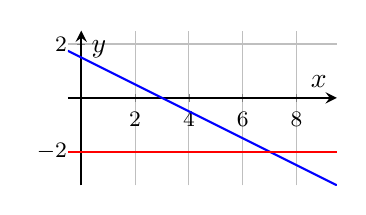
\begin{tikzpicture}[]
\begin{axis}[footnotesize
    , axis equal image, axis lines=middle,
    , xlabel={$x$},ylabel={$y$}, thick, no marks, grid, ymax=2.5
    , domain=-0.5:9.5 ]
    \addplot{(3-x)/2};
    \addplot{-2+0*x};
\end{axis}
\end{tikzpicture}}%
although there are two leading ones multiplying \(x\) and~\(y\) in the first and the second equation respectively, the variable~\(y\) does not have zero coefficients in the first equation.  
(A solution to this system exists, shown  in the margin, but the question does not ask for it.)
\end{solution}

\item \(\begin{bmatrix} -1&4&1&6\V-1
\\3&0&1&-2\V-2
 \end{bmatrix}\)
\begin{solution} 
This augmented matrix is not in \rref\ as there are no leading ones. 
\end{solution}
\end{enumerate}
\end{example}



\begin{activity}
Which one of the following augmented matrices is \emph{not} in \idx{reduced row echelon form}?
\actposs{\(\begin{bmatrix} 1&1&0\V0
\\0&-1&1\V-1 \end{bmatrix}\)}
{\(\begin{bmatrix} 1&0&1\V2
\\0&1&0\V1 \end{bmatrix}\)}
{\(\begin{bmatrix} 0&1&1\V-1
\\0&0&0\V0 \end{bmatrix}\)}
{\(\begin{bmatrix} 0&1&0\V1
\\0&0&1\V2 \end{bmatrix}\)}
\end{activity}





\begin{activity}
Which one of the following is a \idx{general solution} to the system with \idx{augmented matrix} in \idx{reduced row echelon form} of
\begin{equation*}
\begin{bmatrix} 1&0&-0.2\V0.4
\\0&1&-1.2\V-0.6 \end{bmatrix}?
\end{equation*}
\actposs{\((0.2t+0.4,1.2t-0.6,t)\)}
{\((0.4,-0.6,0)\)}
{\((0.2+0.4t,1.2+0.6t,t)\)}
{solution does not exist}
\end{activity}



The previous \autoref{eg:rref} shows that given a system of linear equations in \idx{reduced row echelon form} we can either immediately write down all solutions, or immediately determine if none exists.
Generalizing \autoref{eg:erowops}, the following Gauss--Jordan procedure uses elementary row operations (\autoref{thm:erowop}) to find an equivalent system of equations in \idx{reduced row echelon form}. 
From such a form we then write down a general solution.




\needspace{7\baselineskip}
\begin{procedure}[\idx{Gauss--Jordan elimination}] \label{pro:gje}
\ \begin{aside}
Computers and graphics calculators perform Gauss--Jordan elimination for you; for example, \verb|A\| in \script. 
However, when \verb|rcond| indicates \verb|A\| is inappropriate, then the \idx{singular value decomposition} of \autoref{sec:fisvd} is a far better choice than such Gauss--Jordan elimination.
\end{aside}\ 
\begin{enumerate}
\item Write down either the full symbolic form of the \idx{system} of \idx{linear equation}s, or the \idx{augmented matrix} of the system of \idx{linear equation}s.
\item Use \idx{elementary row operation}s to reduce the \idx{system}\slash\idx{augmented matrix} to \idx{reduced row echelon form}.
\item If the resulting system is \idx{consistent}, then solve for the leading variables in terms of any remaining \idx{free variable}s to obtain a \bfidx{general solution}.
\end{enumerate}
\end{procedure}



\begin{example} \label{eg:gjea}
Use \idx{Gauss--Jordan elimination}, \autoref{pro:gje}, to find all possible solutions to the system
\begin{equation*}
\begin{array}{l}
-x-y=-3\,,\\x+4y=-1\,,\\2x+4y=c\,,
\end{array}
\end{equation*}
depending upon the parameter~\(c\).

\begin{solution} 
Here write both the full symbolic equations and the augmented matrix form---you would only have to do one.
\begin{eqnarray*}
\begin{cases}
-x-y=-3\\x+4y=-1\\2x+4y=c
\end{cases}
&\iff&%\leftrightarrow&
\begin{bmatrix} -1&-1\V-3\\1&4\V-1\\2&4\V c \end{bmatrix}
\\
\parbox{0.5\linewidth}{Multiply the first by~\((-1)\).}
\\
\begin{cases}
x+y=3\\x+4y=-1\\2x+4y=c
\end{cases}
&\iff&%\leftrightarrow&
\begin{bmatrix} 1&1\V3\\1&4\V-1\\2&4\V c \end{bmatrix}
\\
\parbox{0.5\linewidth}{Subtract the first from the second, and twice the first from the third.}
\\
\begin{cases}
x+y=3\\0x+3y=-4\\0x+2y=c-6
\end{cases}
&\iff&%\leftrightarrow&
\begin{bmatrix} 1&1\V3\\0&3\V-4\\0&2\V c-6 \end{bmatrix}
\\
\parbox{0.5\linewidth}{Divide the second by three.}
\\
\begin{cases}
x+y=3\\0x+y=-\frac43\\0x+2y=c-6
\end{cases}
&\iff&%\leftrightarrow&
\begin{bmatrix} 1&1\V3\\0&1\V-\frac43\\0&2\V c-6 \end{bmatrix}
\\
\parbox{0.5\linewidth}{Subtract the second from the first, and twice the second from the third.}
\\
\begin{cases}
x+0y=\frac{13}3\\0x+y=-\frac43\\0x+0y=c-\frac{10}3
\end{cases}
&\iff&%\leftrightarrow&
\begin{bmatrix} 1&0\V\frac{13}3\\0&1\V-\frac43\\0&0\V c-\frac{10}3 \end{bmatrix}
\end{eqnarray*}
The system is now in reduced row echelon form.
The last row immediately tells us that there is no solution for parameter \(c\neq\frac{10}3\) as the equation would then be inconsistent.
If parameter \(c=\frac{10}3\)\,, then the system is consistent and the first two rows give that the only solution is \((x,y)=(\frac{13}3,-\frac43)\).
\end{solution}
\end{example}



\begin{example} \label{eg:gjeb}
Use \idx{Gauss--Jordan elimination}, \autoref{pro:gje}, to find all possible solutions to the  system
\begin{equation*}
\begin{cases}
-2v+3w=-1\,,\\2u+v-w=-1\,.
\end{cases}
\end{equation*}

\begin{solution} 
Here write both the full symbolic equations and the augmented matrix form---you would choose one or the other representations.
\begin{eqnarray*}
\begin{cases}
0u-2v+3w=-1\\2u+v-w=-1
\end{cases}
&\iff&%\leftrightarrow&
\begin{bmatrix} 0&-2&3\V-1\\2&1&1\V-1 \end{bmatrix}
\\
\parbox{0.5\linewidth}{Swap the two rows to get a nonzero top-left entry.}
\\
\begin{cases}
2u+v-w=-1\\0u-2v+3w=-1
\end{cases}
&\iff&%\leftrightarrow&
\begin{bmatrix} 2&1&-1\V-1\\0&-2&3\V-1 \end{bmatrix}
\\
\parbox{0.5\linewidth}{Divide the first row by two.}
\\
\begin{cases}
u+\frac12v-\frac12w=-\frac12\\0u-2v+3w=-1
\end{cases}
&\iff&%\leftrightarrow&
\begin{bmatrix} 1&\frac12&-\frac12\V-\frac12\\0&-2&3\V-1 \end{bmatrix}
\\
\parbox{0.5\linewidth}{Divide the second row by~\((-2)\).}
\\
\begin{cases}
u+\frac12v-\frac12w=-\frac12\\0u+v-\frac32w=\frac12
\end{cases}
&\iff&%\leftrightarrow&
\begin{bmatrix} 1&\frac12&-\frac12\V-\frac12\\0&1&-\frac32\V\frac12 \end{bmatrix}
\\
\parbox{0.5\linewidth}{Subtract half the second row from the first.}
\\
\begin{cases}
u+0v+\frac14w=-\frac34\\0u+v-\frac32w=\frac12
\end{cases}
&\iff&%\leftrightarrow&
\begin{bmatrix} 1&0&\frac14\V-\frac34\\0&1&-\frac32\V\frac12 \end{bmatrix}
\end{eqnarray*}
The system is now in reduced row echelon form.  
The third column is that of a free variable so set the third component \(w=t\) for arbitrary~\(t\).
Then the first row gives \(u=-\frac34-\frac14t\)\,, and the second row gives \(v=\frac12+\frac32t\)\,.
That is, the solutions are \((u,v,w)=(-\frac34-\frac14t,\frac12+\frac32t,t)\) for arbitrary~\(t\).
\end{solution}
\end{example}




\subsection{Three possible numbers of solutions}
\label{sec:3pns}

The number of possible solutions to a system of equations is fundamental.  
We need to know all the possibilities.
As seen in previous examples, the following theorem says there are only three possibilities for linear equations.

\begin{theorem} \label{thm:fred}
For every system of linear equations \(A\xv=\bv\)\,, exactly one of the following is true:
\begin{itemize}
\item there is \idx{no solution};
\item there is a \idx{unique solution};
\item there are \idx{infinitely many solutions}.
\end{itemize}
\end{theorem}

\begin{comment}
After studying \autoref{sec:svdsgs}, this theorem could alternatively be proved directly from the use of the so-called \idx{singular value decomposition} in solving the linear equation \(A\xv=\bv\)\,.
\end{comment}

\begin{proof} 
First, if there is exactly none or one solution to \(A\xv=\bv\), then the theorem holds. 
Second, suppose there are two distinct solutions; let them be \(\yv\) and~\(\zv\) so \(A\yv=\bv\) and \(A\zv=\bv\).  
Then consider \(\xv=t\yv+(1-t)\zv\) for all~\(t\) (a parametric description of the line through~\yv\ and~\zv, \autoref{sec:pel}). 
%By distributivity \(A\xv=A(t\xv_1+(1-t)\xv_2) =tA\xv_1+(1-t)A\xv_2 =t\bv+(1-t)\bv =t\bv+\bv-t\bv =\bv\).  
Consider the first row of~\(A\xv\): by \autoref{def:matvecsys} it is
\begin{eqnarray*}&&
a_{11}x_1+a_{12}x_2+\cdots+a_{1n}x_n
\\&=&a_{11}[ty_1+(1-t)z_1]+a_{12}[ty_2+(1-t)z_2]
\\&&{}
+\cdots+a_{1n}[ty_n+(1-t)z_n]
\\&&\quad(\text{then rearrange this scalar expression})
\\&=&t[a_{11}y_1+a_{12}y_2+\cdots+a_{1n}y_n]
\\&&{}
+(1-t)[a_{11}z_1+a_{12}z_2+\cdots+a_{1n}z_n]
\\&=&t[\text{first row of }A\yv]
+(1-t)[\text{first row of }A\zv]
\\&=&tb_1+(1-t)b_1 \quad(\text{as }A\yv=\bv\text{ and }A\zv=\bv)
\\&=&b_1\,.
\end{eqnarray*}
Similarly for all rows of~\(A\xv\): that is, each row in \(A\xv\) equals the corresponding element of~\bv.
Consequently, \(A\xv=\bv\) for all~\(t\). 
Hence, if there are ever two distinct solutions, then there are an infinite number of solutions: \(\xv=t\yv+(1-t)\zv\) for all~\(t\).
\end{proof}




An important class of linear equations always has at least one solution, never none.
For example, modify \autoref{eg:gjea} to 
\begin{equation*}
\begin{array}{l}
-x-y=0\,,\\x+4y=0\,,\\2x+4y=0\,,
\end{array}
\end{equation*}
and then \(x=y=0\) is immediately a solution.  
The reason is that the right-hand side is all zeros and so \(x=y=0\) makes the left-hand sides also zero.

\begin{definition} \label{def:homosys} 
A system of \idx{linear equation}s is called \bfidx{homogeneous} if the (right-hand side) \idx{constant term} in each equation is \idx{zero}; that is, when the system may be written \(A\xv=\ov\)\,.
Otherwise the system is termed \bfidx{non-homogeneous}.
\end{definition}

\begin{example} \label{eg:homosys}
\ 
\begin{enumerate}[ref=\ref{eg:homosys}(\alph*)]
\item\label[example]{eg:homosysi} 
\(\begin{cases}
3x_1-3x_2=0\\-x_1-7x_2=0
\end{cases}\) is homogeneous.  
Solving, the first equation gives \(x_1=x_2\) and substituting in the second then gives \(-x_2-7x_2=0\) so that \(x_1=x_2=0\) is the only solution.
It must have \(\xv=\ov\) as a solution as the system is homogeneous.
 
\begin{reduce}
\item \(\begin{cases}
2r+s-t=0\\ r+s+2t=0\\-2r+s=3\\2r+4s-t=0
\end{cases}\) is not homogeneous because there is a nonzero constant on the right-hand side.
\end{reduce}
 
\item \(\begin{cases}
-2+y+3z=0\\2x+y+2z=0
\end{cases}\) is not homogeneous because there is a nonzero constant in the first equation, the~\((-2)\), even though it is here sneakily written on the left-hand side.
 
\item \label[example]{eg:homosysiv} 
\(\begin{cases}
x_1+2x_2+4x_3-3x_4=0\\
x_1+2x_2-3x_3+6x_4=0
\end{cases}\) is homogeneous.  
Use \idx{Gauss--Jordan elimination}, \autoref{pro:gje}, to solve: 
\begin{eqnarray*}
\begin{cases}
x_1+2x_2+4x_3-3x_4=0\\
x_1+2x_2-3x_3+6x_4=0
\end{cases}
&\iff&%\leftrightarrow&
\begin{bmatrix} 1&2&4&-3\V0
\\1&2&-3&6\V0
 \end{bmatrix}
\\
\parbox{0.5\linewidth}{Subtract the first row from the second.}
\\
\begin{cases}
x_1+2x_2+4x_3-3x_4=0\\
0x_1+0x_2-7x_3+9x_4=0
\end{cases}
&\iff&%\leftrightarrow&
\begin{bmatrix} 1&2&4&-3\V0
\\0&0&-7&9\V0
 \end{bmatrix}
\\
\parbox{0.5\linewidth}{Divide the second row by~\((-7)\).}
\\
\begin{cases}
x_1+2x_2+4x_3-3x_4=0\\
0x_1+0x_2+x_3-\frac97x_4=0
\end{cases}
&\iff&%\leftrightarrow&
\begin{bmatrix} 1&2&4&-3\V0
\\0&0&1&-\frac97\V0
 \end{bmatrix}
\\
\parbox{0.5\linewidth}{Subtract four times the second row from the first.}
\\
\begin{cases}
x_1+2x_2+0x_3+\frac{15}7x_4=0\\
0x_1+0x_2+x_3-\frac97x_4=0
\end{cases}
&\iff&%\leftrightarrow&
\begin{bmatrix} 1&2&0&\frac{15}7\V0
\\0&0&1&-\frac97\V0
 \end{bmatrix}
\end{eqnarray*}
The system is now in reduced row echelon form.  
The second and fourth columns are those of \idx{free variable}s so set the second and fourth component \(x_2=s\) and \(x_4=t\) for arbitrary \(s\) and~\(t\).
Then the first row gives \(x_1=-2s-\frac{15}7t\)\,, and the second row gives \(x_3=\frac97t\)\,.
That is, the solutions are \(\xv=(-2s-\frac{15}7t,s,\frac97t,t) =(-2,1,0,0)s+(-\frac{15}7,0,\frac97,1)t\) for arbitrary \(s\) and~\(t\).
These solutions include \(\xv=\ov\) via the choice \(s=t=0\).
\end{enumerate}
\end{example}




\begin{activity}
Which one of the following systems of equations for \(x\) and~\(y\) is \idx{homogeneous}?
\actposs{\(5y=3x\) and \(4x=2y\)}
{\(-3x-y=0\) and \(7x+5y=3\)}
{\(3x+1=0\) and \(-x-y=0\)}
{\(-2x+y-3=0\) and \(x+4=2y\)}
\end{activity}





As \autoref{eg:homosysiv} illustrates, a further subclass of homogeneous systems is immediately known to have an infinite number of solutions.
Namely, if the number of equations is less than the number of unknowns (two is less than four in \autoref{eg:homosysiv}), then a homogeneous system always has an infinite number of solutions.


\begin{theorem} \label{thm:feweqns} 
If \(A\xv=\ov\) is a \idx{homogeneous} system of \(m\)~\idx{linear equation}s with \(n\)~variables where \(m<n\)\,, then the system has \idx{infinitely many solutions}.
\end{theorem}

Remember that this theorem says nothing about the cases where there are at least as many equations as variables (\(m\geq n)\), when there may or may not be an infinite number of solutions.

\begin{proof} 
The zero vector, \(\xv=\ov\) in~\(\RR^n\), is a solution of \(A\xv=\ov\) so a homogeneous system is always consistent.
In the reduced row echelon form there are at most \(m\)~leading variables---one for each row.
Here \(n>m\) and so the number of free variables is at least \(n-m>0\)\,.
Hence there is at least one free variable and consequently an infinite number of solutions.
\end{proof}

%After studying \autoref{sec:svdsgs}, this theorem could also be proved directly from the use of the so-called \idx{singular value decomposition} in solving the homogeneous linear equation \(A\xv=\ov\)\,.



\paragraph{Prefer a matrix/vector level}
\begin{quoted}{\cite[\S2]{Higham2015b}}
Working at the element level in this way leads to a profusion of symbols, superscripts, and subscripts that tend to obscure the mathematical structure and hinder insights being drawn into the underlying process.
One of the key developments in the last century was the recognition that it is much more profitable to work at the matrix level.
\end{quoted}

A large part of this and preceding sections is devoted to arithmetic and algebraic manipulations on the individual coefficients and variables in the system. 
This is working at the `element level' commented on by Higham.
But as Higham also comments, we need to work more at a whole matrix level.
This means we need to discuss and manipulate matrices as a whole, not  get enmeshed in the intricacies of the element operations.
This has close intellectual parallels in computing where abstract data structures empower us to encode complex tasks: here the analogous abstract data structures are matrices and vectors, and working with matrices and vectors as objects in their own right empowers linear algebra.
The next chapter proceeds to develop linear algebra at the matrix level.

But first, the next \autoref{sec:lcss} establishes some necessary fundamental aspects at the vector level.




\sectionExercises


\begin{exercise} \label{ex:somsys} 
For each of the following systems, write down two different \idx{matrix-vector form}s of the equations.  
For each system: how many different possible matrix-vector forms could be written down?
% Do not reorder or change without changing the next exercise
\begin{Parts}
\item\label{ex:somsysa} \(\begin{array}{l}
-3x+6y=-6\\
-x-3y=4
\end{array}\)
\answer{e.g. \(\protect\begin{bmat} -3&6\protect\\-1&-3 \protect\end{bmat}
\protect\begin{bmat} x\protect\\y \protect\end{bmat}
=\protect\begin{bmat} -6\protect\\4 \protect\end{bmat}\),
\(\protect\begin{bmat} 6&-3\protect\\-3&-1 \protect\end{bmat}
\protect\begin{bmat} y\protect\\x \protect\end{bmat}
=\protect\begin{bmat} -6\protect\\4 \protect\end{bmat}\).
Four: two orderings of rows, and two orderings of the variables.}

\item \(\begin{array}{l}
-2p-q+1=0\\
p-6q=2
\end{array}\)
\answer{e.g. \(\protect\begin{bmat} -2&-1\protect\\1&-6 \protect\end{bmat}
\protect\begin{bmat} p\protect\\q \protect\end{bmat}
=\protect\begin{bmat} -1\protect\\2 \protect\end{bmat}\),
\(\protect\begin{bmat} 1&-6\protect\\-2&-1 \protect\end{bmat}
\protect\begin{bmat} p\protect\\q \protect\end{bmat}
=\protect\begin{bmat} 2\protect\\-1 \protect\end{bmat}\).
Four: two orderings of rows, and two orderings of the variables.}

\item \(\begin{array}{l}
   7.9x  -4.7y=  -1.7\\
   2.4x  -0.1y=   1\\
  -3.1x  +2.7y=   2.3\end{array}\)
\answer{Twelve possibilities: \(3!=6\) orderings of rows, and two orderings of the variables.}

\item \(\begin{array}{l}
   3a+   4b-\frac52c=0\\
  -\frac72a+ b  -\frac92c  -\frac92=0
\end{array}\)
\answer{Twelve possibilities: two orderings of rows, and \(3!=6\) orderings of the variables.}

\item \(\begin{array}{l}
   u+v  -2w=  -1\\
  -2u  -v+   2w=   3\\
   u+   v+   5w=   2
\end{array}\)
\answer{36~possibilities: \(3!=6\)  orderings of rows, and \(3!=6\) orderings of the variables.}

\end{Parts}
\end{exercise}


\begin{exercise}  
Use \autoref{pro:unisol} in \script\ to try to solve each of the systems of \autoref{ex:somsys}.
% surprizingly the following works, except arabic instead of alph
\answer{\protect\begin{enumerate}[label=(\protect\alph*)]
\protect\item \((x,y)=(-0.4,-1.2)\)
\protect\item \((p,q)=(0.6154,-0.2308)\)
\protect\item{}No solution as \protect\verb|rcond| requires a square matrix.
\protect\item{}No solution as \protect\verb|rcond| requires a square matrix.
\protect\item \((u,v,w)=(-2,1.8571,0.4286)\)
\protect\end{enumerate}}
\end{exercise}




\begin{exercise} \label{ex:3lineq} 
Use \autoref{pro:unisol} in \script\ to try to solve each of the following systems.
\begin{enumerate}
\item \(\begin{array}{l}
-5x  -3y   +5z=  -3 \\
   2x   +3y  -z = -5\\
  -2x   +3y   +4z=  -3
\end{array}\)
\answer{\((x,y,z)=(-48,17\tfrac23,-38)\)}

\item \(\begin{array}{l}
-p   +2q  -r=  -2\\
  -2p   +q   +2r=   1\\
  -3p   +4q=   4\end{array}\)
\answer{\((p,q,r)=(32,25,20)\)}

\item \(\begin{array}{l}
u   +3v   +2w=  -1\\
      3v   +5w=   1\\
  -u      +3w=   2\end{array}\)
\answer{\(\protect\verb|rcond|=0\) so no answer found.}

\begin{reduce}
\item \(\begin{array}{l}
-4a  -b  -3c=  -2\\
   2a    -4c=   4\\
   a     -7c=  -2\end{array}\)
\answer{\((a,b,c)=(3.6,-14.8,0.8)\)}
\end{reduce}

%\item \(\begin{array}{l}
%\end{array}\)
%\begin{answer}
%\(\)
%\end{answer}
%
\end{enumerate}
\end{exercise}


\begin{exercise}  
Use \idx{elementary row operation}s (\autoref{thm:erowop}) to solve the systems in \autoref{ex:3lineq}.
\answer{As before, except \((u,v,w)=(-2+3t,\tfrac13-\tfrac53t,t\) for all~\(t\).}
\end{exercise}





\begin{exercise}  
Use \autoref{pro:unisol} in \script\ to try to solve each of the following systems.
\begin{enumerate}
\item \(\begin{array}{l}
2.2x_1  -2.2x_2  -3.5x_3  -2.2x_4=   2.9\\
   4.8x_1+   1.8x_2  -3.1x_3  -4.8x_4=  -1.6\\
  -0.8x_1+   1.9x_2  -3.2x_3+   4.1x_4=  -5.1\\
  -9x_1+   3.5x_2  -0.7x_3+   1.6x_4=  -3.3\end{array}\)
\answer{\(\xv=(-0.26,
  -1.33,
   0.18,
  -0.54)\) \twodp}

\item \(\begin{array}{l}
   0.7c_1+   0.7c_2+   4.1c_3  -4.2c_4=  -0.70\\
   c_1+  c_2+  2.1c_3 -5.1c_4= -2.8\\
   4.3c_1+  5.4c_2+  0.5c_3+  5.5c_4= -6.1\\
  -0.6c_1+  7.2c_2+  1.9c_3 -0.6c_4= -0.3\end{array}\)
\answer{\(\cv=(-1.64,
  -0.30,
   0.58,
   0.41)\) \twodp}

%\item \(\begin{array}{l}
%\end{array}\)
%\begin{answer}
%\(\)
%\end{answer}
%
\end{enumerate}
\end{exercise}





\begin{exercise}  
Each of the following show some \script\ commands and their results.
Write down a possible problem that these commands aim to solve, and interpret what the results mean for the problem.
\begin{enumerate}
\item
\begin{verbatim}
>> A=[0.1 -0.3; 2.2 0.8]
A =
   0.1000  -0.3000
   2.2000   0.8000
>> b=[-1.2; 0.6]
b =
  -1.2000
   0.6000
>> rcond(A)
ans =  0.1072
>> x=A\b
x =
  -1.054
   3.649
\end{verbatim}
\answer{Solve the system \(0.1x-0.3y=-1.2\), \(2.2x+0.8y=0.6\).
Since \protect\verb|rcond| is good, the solution is \(x=-1.05\), \(x_2=0.63\) and \(y=3.65\) \twodp.}

\begin{reduce}
\item 
\begin{verbatim}
>> A=[1.1 2 5.6; 0.4 5.4 0.5; 2 -0.2 -2.8]
A =
    1.1000    2.0000    5.6000
    0.4000    5.4000    0.5000
    2.0000   -0.2000   -2.8000
>> b=[-3;2.9;1]
b =
   -3.0000
    2.9000
    1.0000
>> rcond(A)
ans =
    0.2936
>> x=A\b
x =
   -0.3936
    0.6294
   -0.6832
\end{verbatim}
\answer{Solve the system \(1.1x_1+2x_2+5.6x_3=-3\), \(0.4x_1+5.4x_2+0.5x_3=2.9\), \(2x_1-0.2x_2-2.8x_3=1\).
Since \protect\verb|rcond| is good, the solution is \(x_1=-0.39\), \(x_2=0.63\) and \(x_3=-0.68\) \twodp.}
\end{reduce}


\item \index{error:@\texttt{error:}}
\begin{verbatim}
>> A=[0.7 1.4; -0.5 -0.9; 1.9 0.7]
A =
   0.7000   1.4000
  -0.5000  -0.9000
   1.9000   0.7000
>> b=[1.1; -0.2; -0.6]
b =
   1.1000
  -0.2000
  -0.6000
>> rcond(A)
error: rcond: matrix must be square
>> x=A\b
x =
  -0.6808
   0.9751
\end{verbatim}
\answer{Fails to solve the system \(0.7x_1+1.4x_2=1.1\), \(-0.5x_1-0.9x_2=-0.2\), \(1.9x_1+0.7x_2=-0.6\) because the matrix is not square as reported by \protect\verb|rcond|.  
The 'answer'~\protect\verb|x| is not relevant (yet).}

\begin{reduce}
\item
\begin{verbatim}
>> A=[-0.7 1.8 -0.1; -1.3 0.3 1.7; 1.8 1. 0.3]
A =
  -0.7000   1.8000  -0.1000
  -1.3000   0.3000   1.7000
   1.8000   1.0000   0.3000
>> b=[-1.1; 0.7; 0.2]
b =
  -1.1000
   0.7000
   0.2000
>> rcond(A)
ans =  0.3026
>> x=A\b
x =
   0.2581
  -0.4723
   0.6925
\end{verbatim}
\answer{Solve the system \(-0.7x+1.8y-0.1z=-1.1\), \(-1.3x+0.3y+1.7z=0.7\), \(1.8x+y+0.3z=0.2\).
Since \protect\verb|rcond| is good, the solution is \(x=0.26\), \(y=-0.47\) and \(z=0.69\) \twodp.}
\end{reduce}


\item
\begin{verbatim}
>> A=[-2 1.2 -0.8; 1.2 -0.8 1.1; 0 0.1 -1]
A =
  -2.0000   1.2000  -0.8000
   1.2000  -0.8000   1.1000
   0.0000   0.1000  -1.0000
>> b=[0.8; -0.4; -2.4]
b =
   0.8000
  -0.4000
  -2.4000
>> rcond(A)
ans =  0.003389
>> x=A\b
x =
   42.44
   78.22
   10.22
\end{verbatim}
\answer{Solve the system \(-2x+1.2y-0.8z=0.8\), \(1.2x-0.8y+1.1z=-0.4\), \(0.1y-z=-2.4\).
Since \protect\verb|rcond| is poor, the reported solution \(x=42.22\), \(y=78.22\) and \(z=10.22\) \twodp\ is suspect (the relatively large magnitude of \((x,y,z)\) is also suspicious).}



\item 
\begin{verbatim}
>> A=[0.3 0.6 1.7 -0.3
-0.2 -1 0.2 1.5
0.2 -0.8 1 1.3
1.2 0.8 -1.1 -0.9]
A =
   0.3000   0.6000   1.7000  -0.3000
  -0.2000  -1.0000   0.2000   1.5000
   0.2000  -0.8000   1.0000   1.3000
   1.2000   0.8000  -1.1000  -0.9000
>> b=[-1.5; -1.3; -2; 1.2]
b =
  -1.500
  -1.300
  -2.000
   1.200
>> rcond(A)
ans =  0.02162
>> x=A\b
x =
  -0.3350
  -0.3771
  -0.8747
  -1.0461
\end{verbatim}
\answer{Solve the system \(0.3x_1 +0.6x_2 +1.7x_3 -0.3x_4=-1.5\),
\(-0.2x_1 -x_2 +0.2x_3 +1.5x_4=-1.3\),
\(0.2x_1 -0.8x_2 +x_3 +1.3x_4=-2\),
\(1.2x_1 +0.8x_2 -1.1x_3 -0.9x_4=1.2\).
Since \protect\verb|rcond| is good, the solution is \(x_1=-0.34\), \(x_2=-0.38\), \(x_3=-0.87\) and \(x_4=-1.05\) \twodp.}

\item \index{error:@\texttt{error:}}
\begin{verbatim}
>> A=[1.4 0.9 1.9; -0.9 -0.2 0.4]
A =
   1.4000   0.9000   1.9000
  -0.9000  -0.2000   0.4000
>> b=[-2.3; -0.6]
b =
  -2.3000
  -0.6000
>> rcond(A)
error: rcond: matrix must be square
>> x=A\b
x =
   0.1721
  -0.2306
  -1.2281
\end{verbatim}
\answer{Fails to solve the system \(1.4x +0.9y +1.9z=-2.3\), \(-0.9x -0.2y +0.4z=-0.6\) as \protect\verb|rcond| tells us the system is not square.  The `answer'~\protect\verb|x| is not relevant (yet).}

\item 
\begin{verbatim}
>> A=[0.3 0.3 0.3 -0.5
 1.5 -0.2 -1 1.5
 -0.6 1.1 -0.9 -0.4
 1.8 1.1 -0.9 0.2]
A =
   0.3000   0.3000   0.3000  -0.5000
   1.5000  -0.2000  -1.0000   1.5000
  -0.6000   1.1000  -0.9000  -0.4000
   1.8000   1.1000  -0.9000   0.2000
>> b=[-1.1; -0.7; 0; 0.3]
b =
  -1.1000
  -0.7000
   0.0000
   0.3000
>> rcond(A)
ans = 5.879e-05
>> x=A\b
x =
   -501.5000
   1979.7500
   1862.2500
   2006.5000
\end{verbatim}
\answer{Solves the system
\(0.3x_1 +0.3x_2 +0.3x_3 -0.5x_4=-1.1\),
\( 1.5x_1 -0.2x_2 -x_3 +1.5x_4=-0.7\),
\( -0.6x_1 +1.1x_2 -0.9x_3 -0.4x_4=0\),
\( 1.8x_1 +1.1x_2 -0.9x_3 +0.2x_4=0.3\).
But since \protect\verb|rcond| is bad, the `answer'~\protect\verb|x| is likely to be meaningless: here the large values \(\xv=(-501.5,1979.75,1862.25,2006.5)\) also suggest a bad answer.}

\begin{comment}
\begin{verbatim}
m=round(2+2*rand),n=round(2+2*rand)
for it=1:999,A=0+round(randn(m,n)*10)/10; 
    if rcond(A)<1e-4, break, end, end, 
A=A
b=0+round(randn(m,1)*10)/10
rcond(A)
x=A\b
\end{verbatim}
\end{comment}

\end{enumerate}
\end{exercise}






\begin{exercise}  
Which of the following systems are in \idx{reduced row echelon form}?
For those that are, determine all solutions, if any.
\begin{enumerate}
\item \(\begin{array}{l}
x_1=-194\\
x_2=564\\
x_3=-38\\
x_4=275
\end{array}\)
\answer{Yes, \(\xv=(-194,564,-38,275))\)}

\item \(\begin{array}{l}
y_1-13.3y_4=-13.1\\
y_2+6.1y_4=5.7\\
y_3+3.3y_4=3.1
\end{array}\)
\answer{Yes, \(\yv=(-13.1+13.3t,5.7-6.1t,3.1-3.3t,t)\) for all~\(t\)}

\item \(\begin{array}{l}
z_1-13.3z_3=-13.1\\
z_2+6.1z_3=5.7\\
3.3z_3+z_4=3.1
\end{array}\)
\answer{Not in \rref\ (unless we reorder the variables).}

\item \(\begin{array}{l}a-d=-4\\
b-\frac72d=-29\\
c-\frac14d=-\frac72
\end{array}\)
\answer{Yes.  \((a,b,c,d)=(-4+t,-29+\frac72t,-\frac72+\frac14t,t)\) for all~\(t\)}

\begin{reduce}
\item \(\begin{array}{l}x+0y=0\\
0x+y=0\\
0x+0y=1\\
0x+0y=0
\end{array}\)
\answer{Yes.  There is no solution as the third equation, \(0=1\), cannot be true.}

\item \(\begin{array}{l}x+0y=-5\\
0x+y=1\\
0x+0y=3
\end{array}\)
\answer{Not in \rref\ as the last does not have a leading one.}
\end{reduce}

%\item \(\begin{array}{l}
%\end{array}\)
%\begin{answer}
%
%\end{answer}
%
\end{enumerate}
\end{exercise}




\begin{reduce}
\begin{exercise}  
For the following rational expressions, express the task of finding the \idx{partial fraction} decomposition as a system of linear equations.
Solve the system to find the decomposition.  
Record your working.
\begin{enumerate}
\item 
\begin{equation*}
\frac{-x^2+2x-5}{x^2(x-1)}
\end{equation*}
\answer{\(-\frac4{x-1}+\frac3x+\frac5{x^2}\)}

\item 
\begin{equation*}
\frac{-4x^3+2x^2-x+2}{(x+1)^2(x-1)^2}
\end{equation*}
\answer{\(-\frac2{x+1}+\frac{9/4}{(x+1)^2}-\frac2{x-1}-\frac1{(x-1)^2}\)}

\item 
\begin{equation*}
\frac{5x^4-x^3+3x^2+10x-1}{x^2(x+2)(x-1)^2}
\end{equation*}
\answer{\(\frac{79/36}{x+2}-\frac{13/9}{x-1}+\frac{16/3}{(x-1)^2} +\frac{17/4}{x}-\frac{1/2}{x^2}\)}


\item 
\begin{equation*}
\frac{4x^4+2x^3-x^2-7x-2}{(x+1)^3(x-1)^2}
\end{equation*}
\answer{\(\frac{19/8}{x-1}-\frac{1/2}{(x-1)^2}+\frac{13/8}{x+1} -\frac{9/4}{(x+1)^2}+\frac{3/2}{(x+1)^3}\)}

\end{enumerate}
\end{exercise}
\end{reduce}





\begin{exercise}  
For each of the following tables of data, use a system of linear equations to determine the nominated polynomial that finds the second column as a function of the first column.
Sketch a graph of your fitted polynomial and the data points.
Record your working.
\begin{Parts}
\item  \(\begin{array}{rr}
\multicolumn2c{\text{linear}}\\\hline
x&y\\\hline
2&-4\\
3&4\\\hline
\end{array}\)
\answer{\(y=8x-20\)}

\item  \(\begin{array}{rr}
\multicolumn2c{\text{quadratic}}\\\hline
x&y\\\hline
-2&-1\\
1&0\\
2&5\\\hline
\end{array}\)
\answer{\(y=-\frac83+\frac32x+\frac76x^2\)}

\item  \(\begin{array}{rr}
\multicolumn2c{\text{quadratic}}\\\hline
p&q\\\hline
0&-1\\
2&3\\
3&4\\\hline
\end{array}\)
\answer{\(q=-1+\frac83p-\frac13p^2\)}

\item  \(\begin{array}{rr}
\multicolumn2c{\text{cubic}}\\\hline
r&t\\\hline
-3&-4\\
-2&0\\
-1&-3\\
0&-6\\\hline
\end{array}\)
\answer{\(t=-6-\frac23t+\frac72t^2+\frac76t^3\)}

%xy=round(randn(4,2)*4),c=[ones(4,1) xy(:,1) xy(:,1).^2 xy(:,1).^3]\xy(:,2)
\end{Parts}
\end{exercise}




\begin{exercise}  
In three consecutive years a company sells goods to the value of \$51M, \$81M and \$92M (in millions of dollars).
Find a quadratic that fits this data, and use the quadratic to predict the value of sales in the fourth year.
\answer{\$84M}
\end{exercise}




\begin{exercise}  
%2011[25] 	10 	98 	34
%2012[26] 	10 	83 	20
%2013[27] 	10 	95 	41
In 2011 there were 98~wolves in Yellowstone National Park; in 2012 there were 83~wolves; and in 2013 there were 95~wolves.
Find a quadratic that fits this data, and use the quadratic to predict the number of wolves in 2014.
To keep the coefficients manageable, write the quadratic in terms of the number of years from the starting year of 2011.
\answer{134~wolves}
\end{exercise}








\begin{exercise} \label{ex:orb4Periods} 
\begin{table}
\caption{\idx{orbital period}s for four \idx{planets} of the \idx{solar system}: the periods are in (Earth) days; the distance is the length of the semi-major axis of the orbits [\idx{Wikipedia}, 2014].}
\label{tbl:orb4Periods}
\begin{equation*}
\begin{array}{p{12ex}rr} \hline
planet&\text{distance}&\text{period}\\
&\text{(Gigametres)}&\text{(days)}\\\hline
Mercury& 57.91 & 87.97 \\
Venus& 108.21 & 224.70 \\
Earth& 149.60& 365.26\\
Mars& 227.94& 686.97\\\hline
%Jupiter& 778.55& 4332.59\\
%Saturn& 1433.45& 10759.22\\
%Uranus& 2870.67& 30687.15\\
%Neptune& 4498.54& 60190.03\\\hline
\end{array}
\end{equation*}
\end{table}%
\autoref{tbl:orb4Periods} lists the time taken by a planet to orbit the Sun and a typical distance of the planet from the Sun. 
Analogous to \autoref{eg:infertemp2}, fit a quadratic polynomial \(T=c_1+c_2R+c_3R^2\) for the period~\(T\) as a function of distance~\(R\).
Use the data for Mercury, Venus and Earth.
Then use the quadratic to predict the period of Mars: what is the error in your prediction?
(\autoref{eg:orbitalPeriods} shows a power law fit is better, and that the power law agrees with \idx{Kepler's law}.)
%\begin{verbatim}
%t=[87.97;224.70;365.26]
%r=[57.91;108.21;149.60]
%A=[ones(3,1) r r.^2]
%rcond(A)
%c=A\t
%tmars=c(1)+c(2)*227.94+c(3)*227.94^2
%relerr=tmars/686.97-1
%\end{verbatim}
% Good conditioning if use units of hundreds of Gm.
\answer{Despite the bad \(\protect\verb|rcond|=6\cdot10^{-6}\), the quadratic reasonably predicts a period for Mars of \(700.63\)~days which is in error by~2\%.}
\end{exercise}







\begin{comment}
Possibly polynomial\slash multivariate curve fitting (exact)  \larsvii{p.25--8} as example of data mining, and scientific and engineering inference? e.g.~discovering `index' combinations.
Applications involving homogeneous systems, such as balance chemical reactions, leave for the next section.
Nakos~\S1.4 has lots of good ideas (including derivation of cosine rule for triangles).
\end{comment}





\begin{exercise}[{Global Positioning System} in space-time] \label{ex:gps3t} 
For each case below, and in space-time, suppose you know from five \gps\ satellites that you and your \gps\ receiver are the given measured time shifts away from the given locations of each of the three satellites (locations are in~Mm).  
Following \autoref{eg:gps3t}, determine both your position and the discrepancy in time between your \gps\ receiver and the satellites \gps\ time.  
Which case needs another satellite?
\begin{enumerate}
\item  
\(\left\{\begin{array}{l@{\text{ time shift before }}l}
0.03\,s&(17,11,17)\\
0.03\,s&(11,20,14)\\
0.0233\cdots\,s&(20,10,9)\\
0.03\,s&(9,13,21)\\
0.03\,s&(7,24,8)
\end{array}\right.\)
\answer{\(\protect\verb|rcond|=0.014\), \((3,4,3)\), shift\({}=12/300=0.04\)\,s}

\item 
\(\left\{\begin{array}{l@{\text{ time shift before }}l}
0.1\,s&(11,12,18)\\
0.1066\cdots\,s&(18,6,19)\\
0.1\,s&(11,19,9)\\
0.1066\cdots\,s&(9,10,22)\\
0.1\,s&(23,3,9)
\end{array}\right.\)
\answer{\(\protect\verb|rcond|=0.034\), \((5,2,3)\), shift\({}=-11/300=-0.0366\cdots\)\,s}

\item 
\(\left\{\begin{array}{l@{\text{ time shift before }}l}
0.03\,s&(17,11,17)\\
0.03\,s&(19,12,14)\\
0.0233\cdots\,s&(20,10,9)\\
0.03\,s&(9,13,21)\\
0.03\,s&(7,24,8)
\end{array}\right.\)
\answer{\(\protect\verb|rcond|=0\), singular, needs another satellite.}

\end{enumerate}
\end{exercise}





\begin{exercise}  
Formulate the following two thousand year old Chinese puzzle as a system of linear equations.
Use algebraic manipulation to solve the system.
\begin{quoted}{Jiuzhang Suanshu, 200\textsc{bc} \cite[p.3]{Chartier2015}}
There are three classes of grain, of which three bundles of the first class, two of the second, and one of the third make 39~measure.
Two of the first, three of the second, and one of the third make 34~measures.
And one of the first, two of the second, and three of the third make 26~measures.
How many measures of grain are contained in one bundle of each class?
\end{quoted}
\answer{\(9\tfrac14\), \(4\tfrac14\) and~\(2\tfrac34\)~measures respectively.}
\end{exercise}



\begin{comment}
Could have project exercises to introduce sensitivity to small errors in applications (experimental computational maths).  
Although sensitivity is quantified in the section on condition number and rank.
\end{comment}





\begin{exercise}  
Suppose you are given data at \(n\)~points, equi-spaced in~\(x\).
Say the known data points are \((1,y_1)\), \((2,y_2)\), \ldots, \((n,y_n)\) for some given \hlist yn.
Seek a polynomial fit to the data of degree~\((n-1)\); that is, seek the fit \(y=c_1+c_2x+c_3x^2+\cdots+c_{n}x^{n-1}\).
In \script, form the matrix of the linear equations that need to be solved for the coefficients \hlist cn.  
According to \autoref{pro:unisol}, for what number~\(n\) of data points is \verb|rcond| good? poor? bad? terrible? 
%a=ones(m,1),for n=2:m, a=[ones(m,1) diag(1:m)*a], rcond(a(1:n,:)), end
\answer{Good, \(\{1,2\}\); poor, \(\{3,4\}\); bad, \(\{5,6,7\}\); terrible, \(\{8,9,\ldots\}\).}
\end{exercise}




\begin{reduce}
\begin{exercise}[\idx{rational function}s]  
%n=5
%x=sort(round(randn(1,n)*6)/2)
%c=round(randn(1,n)*3)
%y=(c(1)+c(2)*x+c(3)*x.^2)./(1+c(4)*x+c(5)*x.^2)
Sometimes we wish to fit rational functions to data.
This fit also reduces to solving linear equations for the coefficients of the rational function.
For example, to fit the rational function \(y=a/(1+bx)\) to data points \((x,y)=(-7,-\frac19)\) and \((x,y)=(2,\frac13)\) we need to satisfy the two equations
\begin{equation*}
-\frac19=\frac a{1-7b} \quad\text{and}\quad
\frac13=\frac a{1+2b}\,.
\end{equation*}
Multiply both sides of each by their denominator to require
\begin{eqnarray*}
&&-\tfrac19(1-7b)= a \quad\text{and}\quad
\tfrac13(1+2b)= a
\\&\iff& a-\tfrac79b=-\tfrac19 \quad\text{and}\quad
a-\tfrac23 b=\tfrac13\,.
\end{eqnarray*}
By hand (or \script) solve this pair of linear equations to find \(a=3\) and \(b=4\)\,.
Hence the required rational function is \(y=3/(1+4x)\).
\begin{enumerate}
\item Similarly, use linear equations to fit the rational function \(y=(a_0+a_1x)/(1+b_1x)\) to the three data points \((1,\tfrac72)\), \((3,\tfrac{19}4)\) and \((4,5)\).
\answer{\(y=(1+6x)/(1+x)\)}

\item Similarly, use linear equations to fit the rational function \(y=(a_0+a_1x+a_2x^2)/(1+b_1x+b_2x^2)\) to the five data points 
\((-\tfrac52,\tfrac{69}{44})\), \((-1,\tfrac{3}2)\), \((\tfrac12,\tfrac98)\), \((1,\tfrac54)\) and \((2,\tfrac{15}{11})\).
\answer{\(y=(1+x+3x^2)/(1+x+2x^2)\)}
\end{enumerate}
\end{exercise}
\end{reduce}



\begin{comment}
Could include exercise(s) on car traffic flow as discussed by Possani et al. (2010).
\end{comment}


\begin{exercise}  
In a few sentences, answer\slash discuss each of the following.
\begin{enumerate}
\item What is the role of the \script\ function \verb|rcond()|?

\item How does the \verb|=|~symbol in \script\ compare with the \(=\)~symbol in mathematics?

\item How can there be several different augmented matrices for a given system of linear equations?  How many different augmented matrices may there be for a system of three linear equations in three unknowns?

\item Why is the reduced row echelon form important?

\item Why cannot there be exactly three solutions to a system of linear equations?

\end{enumerate}
\end{exercise}

\begin{comment}%{ED498555.pdf}
why, what caused X?
how did X occur?
what-if? what-if-not?
how does X compare with Y?
what is the evidence for X?
why is X important?
\end{comment}

\index{linear equation|)}
\index{system|)}

